\documentclass[]{article}

\usepackage{graphicx}

\begin{document}

\title{Amadahl and Gustafson Revisited for Fault Tolerance}
\author{Wesley Bland, George Bosilca, Thomas Herault, Jack Dongarra\\
		\{wbland, bosilca, herault, dongarra\}@eecs.utk.edu\\
		EECS Department, University of Tennessee}
\date{May 8, 2011}

\maketitle

\section{Introduction}
\label{sect:introduction}

%Statements about Amdahl & Gustafson's Laws
In an effort to understand the effect of improving code and the effect of parallelism, Amdahl~\cite{Amdahl:1967up} and Gustafson~\cite{Gustafson:1988p6477} published ideas which became known as Amdahl's Law and Gustafson's Law. These two laws have formed an understanding of the improvement of parallelizing code.

%Statements about faults tolerance
However, these laws are basic and do not take into account considerations such as faults and fault tolerance. As machine sizes increase in the quest for widespread petascale and future exascale systems, the prevalence of faults will only become a larger concern for software engineers. Even with very reliable hardware, statistics and experience show that software must be ready to react to a both hardware and software faults.

%Describe need to re-visualize laws in the face of faults
When these faults inevitably occur, they cause setbacks for the code running on the machine. These result in work either being lost or redone. By including these losses and recalculations into the models presented by Amdahl and Gustafson, users and code designers can gain a better understanding of the expected behavior of their codes.

%Outline paper
Section~\ref{sect:background} of this paper will give a brief overview of the state of fault tolerance in High Performance Computing (HPC). Section~\ref{sect:original} will describe the original laws of Amdahl and Gustafson. Section~\ref{sect:improved} will add consideration of faults and fault recovery to the laws. Section~\ref{sect:results} will discuss the results of these changes to the laws and present graphically the difference that they cause. Finally, section~\ref{sect:conclusion} concludes the paper and summarizes the work that took place.

\section{Background Work}
\label{sect:background}

%Describe big machines, frequency of failures, etc.
HPC systems continue to grow in size. In the most recent Top500\footnote{http://www.top500.org} list, 12 of the top 16 machines had more than 100,000 cores. Each has massive amounts of memory, disk space, networking equipment, cooling, and other hardware parts that can fail. Beyond expected hardware failures, software itself can fail due to coding errors or invalid input. All of these cause unexpected failures that applications must be able to handle. Franck Cappello~\cite{Cappello:2009dd}, looked at data from the ``Computer Failure Data Repository'' and concluded that on some systems at Los Alamos National Laboratory, the Mean Time Between Failures (MTBF) can be a short as 8 hours. This is an alarmingly low number and underscores the necessity of a system to manage these faults without a total application restart.

%Cite other papers about need for fault tolerance
%May or may not add more here

%Describe some approaches to fault tolerance
Many groups attempting to tackle fault tolerance in a variety of ways. Each method of fault tolerance has its merits and the choice of which method to use with a particular application is dependent on the desired results.

%Checkpoint / Restart
Checkpoint / Restart is useful when running on a system with good throughput to disk. It periodically creates a snapshot of the running application and when a failure is detected, it restores the system to a known useful state by loading the checkpoint from stable storage. The drawback of this method is that it requires heavy usage of disk I/O which becomes a performance bottleneck. This problem increases dramatically as the machine size increases. It also requires a sophisticated technique to ensure that the snapshots form a consistent picture of the system at a particular time~\cite{Chandy:1985ip}.

%Run-Through Stabilization
Run-through stabilization is useful in applications that can withstand the loss of one or more nodes without compromising their results. The advantage of this form of fault tolerance is that it requires the least amount of work to recover from a failure. The application simply removes the dead process from whatever internal bookkeeping it uses and continues on with its calculations~\cite{Cappello:2009dd}. However, this solution is not well-suited to many application's needs and often must be used in conjunction with other forms of fault tolerance.

%Restore/Replace Dead Processes
When applications cannot continue after the loss of a process, they must either restore the failed process or replace it with another process. The backup process can be in the form of a ``hot'' replacement which performs the same computations as the primary processes and is ready to be substituted into the application or it can be a ``cold'' replacement that must either start over from the beginning of the application or from a previously saved checkpoint. This form of fault tolerance can incur a significant penalty as any calculations performed by the faulty process must be redone before the application can continue.

\section{Original Laws}
\label{sect:original}

\subsection{Amdahl's Law}
\label{subsect:amdahl_original}

%Describe Amdahl's Law
In 1967 Gene Amdahl introduced the idea that would come to be known as Amdahl's Law~\cite{Amdahl:1967up}. It described the effect of speeding up a section of code without improving the rest of the code. The law showed that even when improving a small section of code dramatically, the runtime of the code is bound by the non-improved sections. The law has been generalized to describe not only improving parts of an application, but also parallelizing an application. The runtime speedup as described by Amdahl's Law is demonstrated by the formula $$\frac{1}{(1-P) + \frac{P}{N}}$$ P describes the portion of the code that is parallelized and N is the number of processors used when running the code.

%Discuss fixed problem size, changing run time
Amdahl's Law describes a situation where the size of a problem does not change as the size of the system it is running on increases. The law only describes the speedup that can be effected by including more processors in the problem's execution.

\subsection{Gustafson's Law}
\label{subsect:gustafson_original}

%Describe Gustafson's Law
21 years later, John Gustafson recognized a flaw in the assumptions of Amdahl's Law~\cite{Gustafson:1988p6477}. Gustafson realized that while academically Amdahl's Law was correct, in practice the applications that it described were not as concerned with fixed size speedup, but would increase the size of the problem to match the machine on which they were executing. He referred to this as a scaled-size model rather than a fixed-sized that Amdahl assumed. Gustafson's Law claimed the speedup could be represented by the formula $$(1-P) + P * N$$ The speedup derived from the fact that the problem size was increasing rather than only a small section of code improving.

\section{Improved Laws}
\label{sect:improved}

\subsection{Amdahl's Law with FT}
\label{subsect:amdahl_improved}

%Amdahl's law assumes recovery
To include a notion of faults into Amdahl's Law, it must be changed to account for process losses in the portion of the computation including the number of participating nodes. Due to the nature of Amdahl's Law, the work that these nodes produce is expected to be recovered as the size of the job is not to be changed based on the size of the machine.

%Show formula
Here we show the improved formula for Amdahl's Law$$\frac{1}{(1-P) + \frac{P}{N_i} (1+\frac{N_f}{N_i})}$$ where $$\ N_f = \frac{\lfloor\frac{R}{MTBF}\rfloor (1 + \lfloor\frac{R}{MTBF}\rfloor)}{2}$$ $N_i$ is the initial number of processes involved in the job and $N_f$ is the fractional number processes that actually participated in the job. The reason this number can be fractional is that it includes the amount of time spent redoing the work of the failed processes.

%C/R can improve things but makes the formula more complicated
There exist optimizations to improve this number. For example, with a checkpoint / restart system, the processes that must be used in recovery could begin from a point closer to the failure or the process they are replacing, thus reducing the amount of work they must perform in order to ``catch up" to the current state of the calculations.

\subsection{Gustafson's Law with FT}
\label{subsect:gustafson_improved}

%Gustafson's law assumes no recovery
Gustafson's Law requires a slightly different approach. While Amdahl's Law assumed recovery from the processes in order to maintain the correct problem size, Gustafson's Law does not share that requirement. Because the runtime is fixed in Gustafson's Law rather than the problem size, there should actually be no recovery and the application should continue without the results of the processes that failed. Monte Carlo simulations would fit into this category of application.

%Show formula
The improved formula for Gustafson's Law is as follows $$(1-P) + P * (N_i - N_f)$$ $N_f$ is the same as in subsection~\ref{subsect:amdahl_improved}. 

\section{Results}
\label{sect:results}

%Graphs of some values plugged into the formulas

\subsection{Amdahl's Law}
\label{subsect:amdahl_results}

\begin{figure}
	\begin{center}
		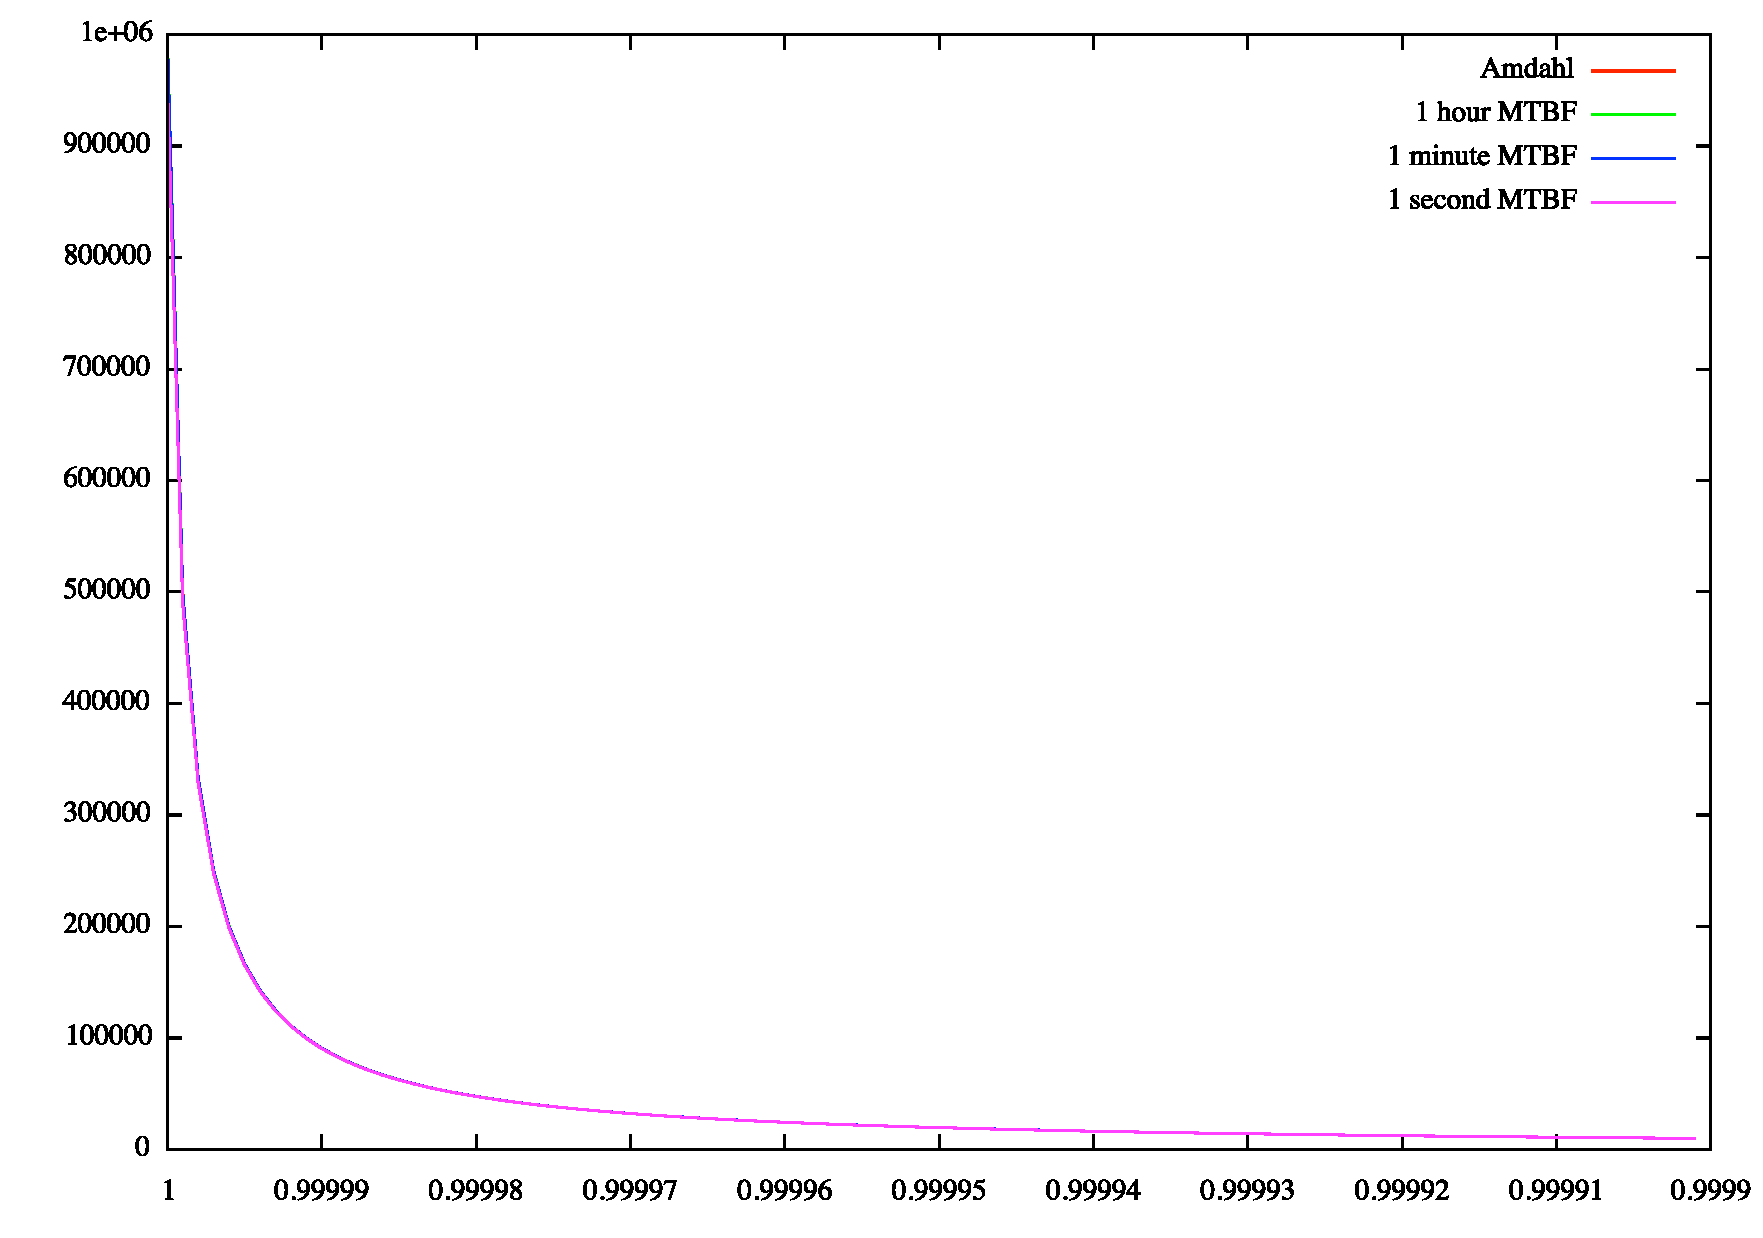
\includegraphics[scale=0.25]{AmdImp.pdf}
		\caption{\small Amdahl's Law with Improvements}
		\label{fig:amdahl_improved}
	\end{center}
\end{figure}

After performing calculations for Amdahl's Law, it was discovered that without creating situations that are unlikely to be realistic in the near future, there was minimal change to the results of the formula. What change did occur was when P was at its maximum, however the difference between the original law and the improved one was dwarfed by the already rapid decrease in speedup derived from the original law. The similarity is shown in figure~\ref{fig:amdahl_improved}. It shows that the change in the result of the formula is minimal because the speedup of the program drops by 90\% almost immediately after introducing any serial code.

%Describe figure
Figure~\ref{fig:amdahl_improved} uses a machine size of 1,000,000. Systems are continually increasing in size and a system size of 1,000,000 is in the near future. With the fastest systems currently at more than 200,000 processing cores, we will reach millions of processing cores within a few years. The runtime used was 24 hours. This is not unreasonable for large codes especially as machine sizes grow. The MTBF was varied between 1 hour and 1 second. This was to show that for Amdahl's Law, there is little difference except at the most extreme values of P.

\subsection{Gustafson's Law}
\label{subsect:gustafson_results}

\begin{figure}
	\begin{center}
		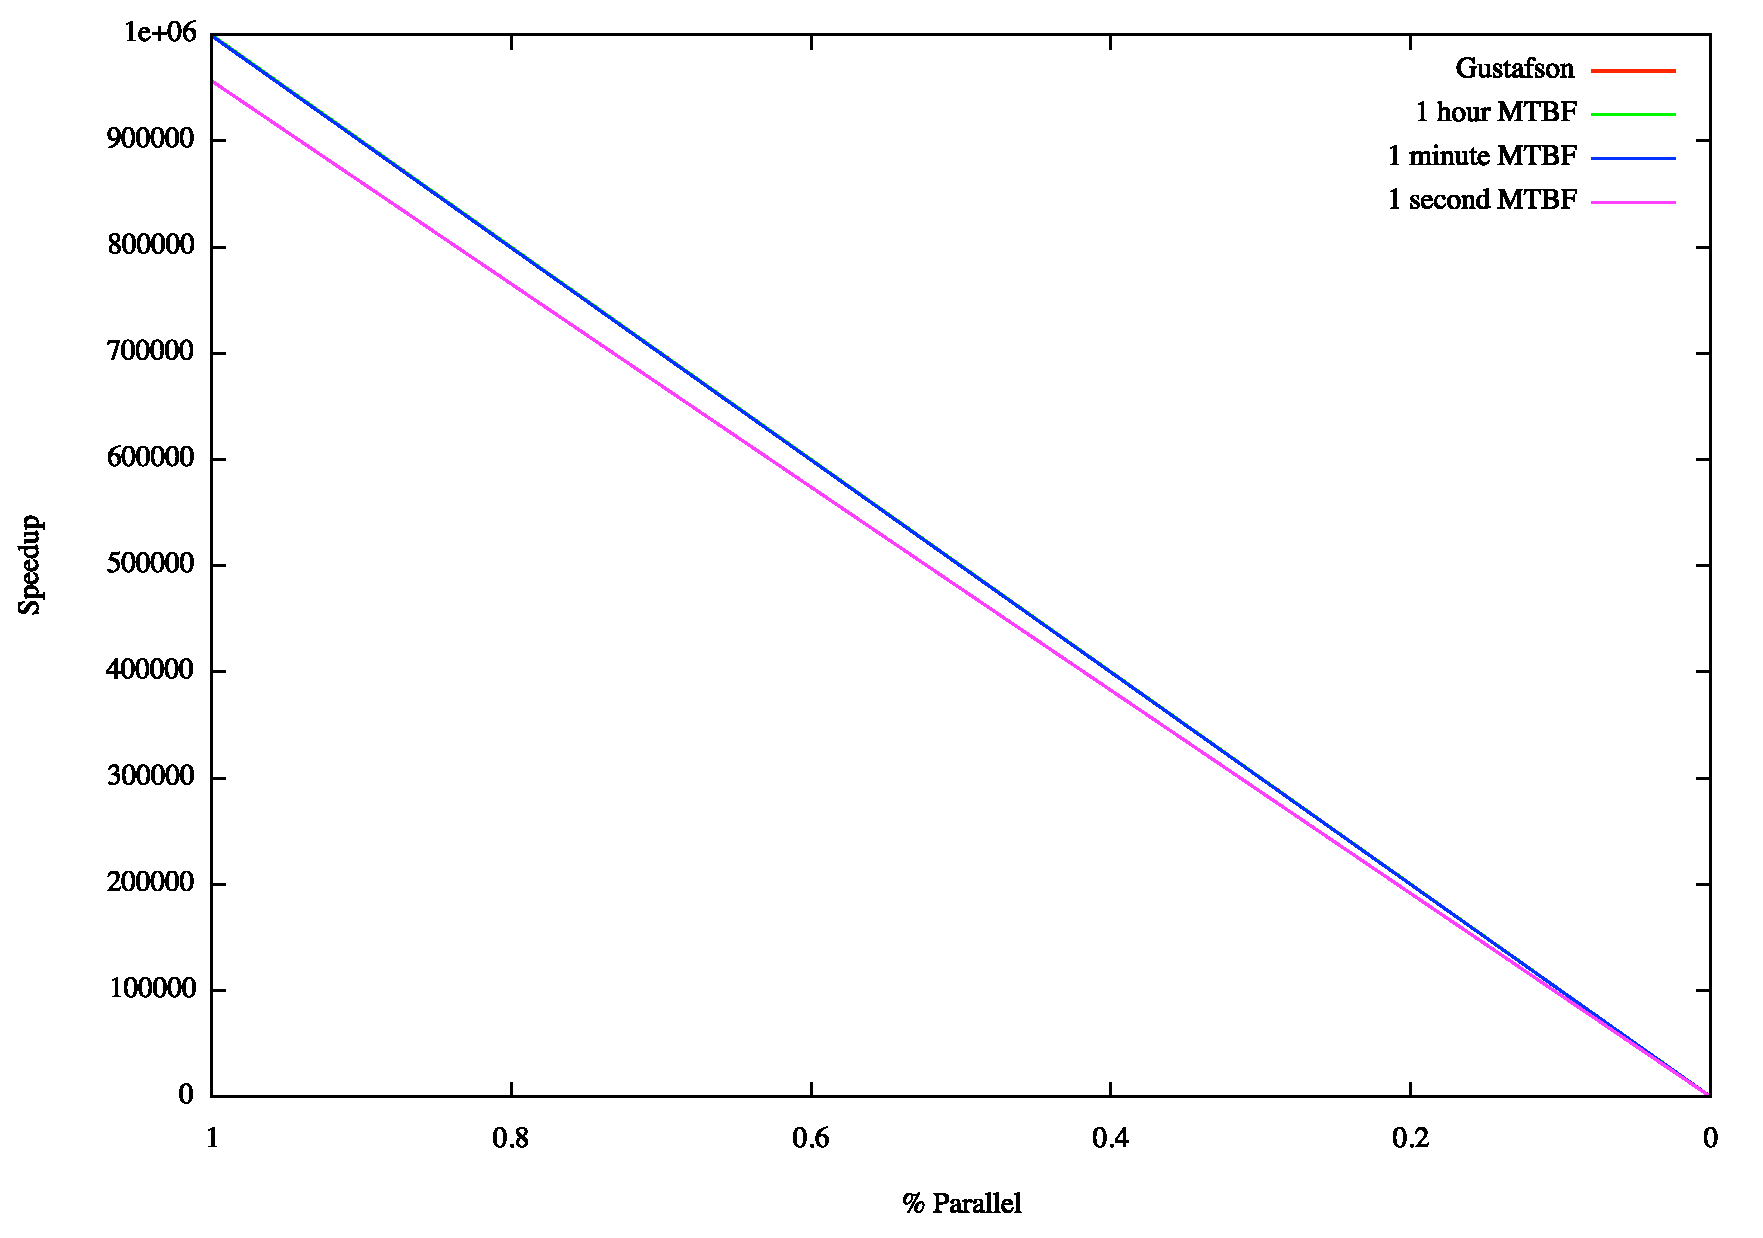
\includegraphics[scale=0.25]{GusImp.pdf}
		\caption{\small Gustafson's Law with Improvements}
		\label{fig:gustafson_improved}
	\end{center}
\end{figure}

Gustafson's Law exhibited similar, but not entirely identical results. Figure~\ref{fig:gustafson_improved} shows that until the MTBF reaches extremely high values, the difference between the original Gustafson Law and the improved version is minor.

%Describe figure
The same input values were used for the Gustafson figure. The machine size is 1,000,000. The runtime is 24 hours, and the MTBF is shown.

\section{Conclusion}
\label{sect:conclusion}

While Amdahl and Gustafson's Laws were written without considering fault tolerance, the difference between including fault tolerance in the formula and not including it is relatively minor. This is good news going forward as it shows that the effect of a few faults will not ruin the speedup gained by increasing the size of the system. However, these improved formulas do not take into account considerations such as fault detection, recovery time, and other overheads that may be incurred by including fault tolerance into HPC. Depending on the quality of the implementations, these could also introduce relatively minor slowdowns or with a poor implementation they could dramatically reduce speedup.

\bibliographystyle{plain}
\bibliography{papers}

\end{document}
